\chapter{脉冲神经网络}
\label{chap:spiking-networks}

前面的网络通常在一次计算中传递实数向量。即使输入是序列，每个时间步也会产生一组连续值表示。如果传感器只在信号变化时报告事件，或者计算设备通过离散脉冲通信，网络还能怎样保留强度、顺序和历史信息？此时，传递了多少次信号、信号何时到达，以及两次信号之间的状态变化，都可能参与计算。

第\ref{chap:neural-network-overview}章介绍了生物神经元通过发放事件通信，第\ref{chap:recurrent-networks}章的液态状态机则展示了固定脉冲储备池与可训练读出的分工。这里进一步追问：怎样把这种通信变为完整的可学习模型？它与连续值网络的差异发生在编码、状态还是连接上，什么任务又值得承担额外的时间模拟与训练成本？

脉冲是通信形式，膜电位是内部状态，两者需要分别建模。只有建立这一区别，才能理解网络为何可以在两次输入之间保留信息，也才能判断少量脉冲是否真的减少了整体计算。以下使用离散时间模型展开可复核的计算，并在需要时说明它与连续时间动态的关系。

\section{脉冲神经网络概述}
\label{sec:snn-overview}

\subsection{提出动机与核心思想}
\label{sec:snn-motivation}

生物细胞的膜电位连续变化，远距离通信却主要通过短暂的动作电位完成。若只用一个实数激活概括活动，就会省略单次发放的时刻、相邻事件的间隔，以及未达到阈值时的内部积累。研究神经计算时，这些信息本身就是要解释的对象；处理变化驱动的传感器时，它们又是输入已经提供的结构。

\term{脉冲神经网络}（spiking neural network, SNN）以离散发放事件在单元之间传递信息，单元内部保存随时间演化的状态。一个脉冲通常只报告某单元在某时刻发放；信号的强度和时序关系由发放次数、发生时刻及发放单元共同承载。接收单元积累这些输入，旧输入逐渐衰减，状态越过阈值时再产生新事件。它既是一种信息编码方式，也是一类带阈值、复位与时间动态的网络模型。

提出这类模型有两条相互联系的动机。一条来自神经科学：用可计算的动态解释细胞如何对输入作出响应，以及局部连接怎样形成行为。另一条来自工程：若变化稀疏，能否只在事件发生时传递和处理必要信息，减少持续感知中的通信与计算？第二条动机要求传感器、编码、模型和执行设备共同配合；仅把实数激活替换成0与1，不能自动得到低能耗系统。

SNN也不要求完全复现生物细胞。模型可以只保留积累、泄漏、阈值和复位，权重可以通过任务损失学习，输出还可以使用连续值读出。这使生物启发与人工任务连接起来，但同时需要分别判断生物解释是否合理、任务预测是否有效，以及实现是否利用了事件稀疏性。

\subsection{从神经元建模到神经形态计算}
\label{sec:snn-early-history}

脉冲网络不是在某一年由一篇论文完整提出的。早期神经元模型、时序编码研究和硬件设计逐步汇合，才形成今天的研究方向。1907年Lapicque的积分发放思想将输入电流的积累与阈值发放联系起来，是早期简化动态模型的一条路线\scite{gerstner2014}

1952年Hodgkin与Huxley从离子电流出发建立动作电位的定量模型。与积分发放模型相比，它解释波形产生机制，说明神经元模型可以在不同生物细节层次上工作：简化模型便于组织较大网络，细致模型则服务于膜电流和发放机制研究\scite{hodgkin1952membrane}

1990年，Mead系统讨论\term{神经形态电子系统}（neuromorphic electronic systems），即借鉴神经系统组织与动态来设计电子计算系统。它关注的不仅是某个神经元方程，还包括局部连接、并行动态和物理实现；神经形态计算的范围因此比某一种SNN模型更广\scite{mead1990neuromorphic}

1997年，Maass以“第三代神经网络模型”讨论脉冲单元的计算能力，把发放时间明确纳入计算。这个代际说法突出阈值单元、连续激活和脉冲时序之间的差异，不表示后出现的模型会在所有任务上取代前面的模型。其表达能力结论依赖编码和单元模型，不能直接换算成真实设备上的精度或能耗优势\scite{maass1997spiking}

脉冲储备池进一步展示了利用复杂动态而不训练全部循环连接的路线。2002年的液态状态机让输入扰动一个固定循环系统，再训练读出使用其动态状态；第\ref{sec:rnn-lsm}节已给出这种分工。局部可塑性则从突触两端活动出发调整连接，为无需完整反向传播的学习提供另一条路径。两者回答的都是“怎样利用时序”，但并不等于解决了任意监督任务的全网信用分配。

\subsection{深层网络与训练方法的发展}
\label{sec:snn-learning-history}

当目标从解释局部动态转为学习多层分类器，离散阈值成为主要困难。2002年，Bohte等提出SpikeProp，根据发放时刻与目标时刻之间的误差进行反向计算；它在特定发放和模型条件下处理时间求导，并不是直接对任意二值脉冲使用普通反向传播\scite{bohte2002spikeprop}

后来的两条路线让深度学习经验更容易进入SNN。一条先训练连续值网络，再校准权重和阈值，使脉冲统计近似原激活；另一条在前向保留离散发放，在反向指定替代导数，直接优化任务损失。第\ref{sec:snn-learning}节会分别说明转换误差和替代梯度的近似性质。2019年的替代梯度综述系统整理了后一条路线，其意义是提供可用的训练信号，而不是消除阈值的不连续性\scite{neftci2019surrogate}

可训练性改善后，研究开始扩展深度与信息交互方式。2021年的SEW-ResNet研究怎样在脉冲残差路径中保持合适的传播；2022年发布、2023年发表于ICLR的Spikformer则将脉冲形式的查询、键和值用于注意力计算。残差与注意力为SNN提供新的组织方式，具体设计仍需检查内部是否保留连续运算、怎样使用时间步，以及哪些操作能映射到目标硬件\scite{fang2021spikingresnet}

Spikformer说明SNN与Transformer不是互斥类别：前者规定事件编码和神经元动态，后者强调信息读取与层间组织。将两者结合，不等于普通Transformer的每个模块都能直接改成脉冲，也不意味着静态图像上的多步推理天然具有事件传感器的稀疏性\scite{zhou2023spikformer}

\subsection{与连续值神经网络的比较}
\label{sec:snn-ann-comparison}

两类网络都可以有前馈、卷积、循环或注意力连接，区别主要在单元输出与时间动态。普通前馈单元一次产生实数激活；脉冲单元先更新内部状态，再决定是否发放。第\ref{sec:rnn-lsm}节的漏积分发放（leaky integrate-and-fire, LIF）单元即使没有循环边，也能用膜电位保存过去输入的影响，而普通逐帧前馈网络通常没有跨帧状态。与RNN比较时，这个差异要收窄：RNN本身也保存状态，SNN额外明确了发放、复位与事件通信。

脉冲也不等同于二值神经网络的低比特激活。二值单元可以在每层计算中输出一个比特，未必具有持续膜电位或有意义的发放时刻；SNN中的0则通常表示这一时间区间没有事件，过去输入仍可能保留在状态中。表~\ref{tab:snn-ann-comparison}按这些机制比较，避免用单个标签概括整套系统。
\begin{table*}[htbp]
  \centering\small
  \begin{tabularx}{\linewidth}{@{}p{25mm}XX@{}}
    \toprule
    比较维度 & 连续值网络 & 脉冲神经网络 \\
    \midrule
    通信变量 & 实数激活或向量 & 发放事件；数量与时刻共同承载信息 \\
    单元内部状态 & 前馈单元通常无跨输入状态；RNN有状态 & 膜电位、突触响应及可选适应状态 \\
    时间关系 & 由递推、位置或时间特征表达 & 由事件时刻、积累、泄漏与延迟表达 \\
    求导困难 & 常见激活可微或分段可微 & 阈值发放不连续，需特别处理 \\
    训练路线 & 任务梯度及其他学习方法 & 局部规则、时间求导、替代梯度或网络转换 \\
    执行成本 & 取决于算子、稀疏性与设备 & 还取决于观察窗口、事件访问和状态更新 \\
    输出形式 & 分类分数、概率或连续量 & 计数、发放时间或连续状态读出 \\
    \bottomrule
  \end{tabularx}
  \caption{以常见人工模型比较两类网络。连续值网络也能使用稀疏计算、动态状态和局部学习；SNN也可能在通用设备上按固定时间步进行稠密计算。表中列出机制差异，不据此给出普遍精度或能耗排序。}
  \label{tab:snn-ann-comparison}
\end{table*}
\FloatBarrier

\subsection{应用现状与发展方向}
\label{sec:snn-development}

事件视觉、稀疏声音或触觉感知、持续监测与机器人响应，是SNN值得研究的场景：输入随时间到达，变化可能稀疏，决策又关心响应延迟。2017年Amir等将事件相机、脉冲识别网络与TrueNorth处理器用于实时手势识别，给出了传感器到设备执行的完整研究系统。这比只在静态图像上报告分类精度更接近事件计算的应用动机，但仍应按其任务、设备和测试条件理解结果\scite{amir2017gesture}

硬件的发展提供了更灵活的实验平台。Loihi面向事件通信、神经元状态和片上学习；Loihi 2进一步支持可编程神经元动态。Intel于2024年公布并部署到Sandia的Hala Point，以Loihi 2构成大规模神经形态研究系统。这里“部署”指研究设施中的系统交付，不能据此推断SNN已成为通用生产工作负载的默认选择\scite{intel2024halapoint}

应用前景取决于完整链路。若输入本来是密集静态图像，需要编码并模拟许多时间步，事件数量和等待时间可能抵消部分收益；若输入是稀疏事件流，输出还需在较短窗口内可靠形成，噪声、低发放量和阈值校准就更关键。把分类结果、能耗估计和实际设备测量分开报告，才能知道改进来自模型、编码还是实现。

已有发展显示两条仍在推进的路线：一条扩大模型的可训练深度、注意力组织和任务范围，另一条围绕稀疏传感器与专用设备共同设计编码、动态和执行方式。由这些研究结果可以提出的判断是，SNN已经具备训练深层任务模型与构造完整实验系统的能力；更广泛的使用仍需要可靠的软件工具、相同条件下的基线比较，以及对状态存储、数据适配和训练成本的控制。这些约束也是后面结构、学习和理论分析需要回答的问题。

\section{网络结构}
\label{sec:snn-coding-dynamics}

脉冲网络由输入编码、带状态的神经元、突触连接和读出组成。连接决定事件送到哪里，神经元动态决定事件到达后留下什么状态、何时产生下一次发放。以下先明确输入事件，再拆开单元内部的计算，随后组合为前馈和循环网络。

\subsection{频率编码与时间编码}
\label{sec:snn-coding}

假设一个传感器在一段时间内观察到某种强度。连续值网络可以直接接收这个数，脉冲网络则需要约定如何把它写进事件序列。对第$i$个输入通道，记发放时刻为$t_{i,k}$。连续时间的脉冲列可以形式化为
\begin{equation}
  s_i(t)=\sum_k\delta(t-t_{i,k})\text{，}
  \label{eq:snn-spike-train}
\end{equation}
其中$\delta$为Dirac脉冲，其意义通过积分给出：对一个只包含某次发放的时间区间积分，得到1。这个表示省略了动作电位的波形，只记录事件时刻。计算机模拟常将时间分为宽度$\Delta t$的$K$个区间，令$s_i^{(t)}\in\{0,1\}$表示第$t$个区间是否发放；若允许同一区间多次发放，变量就应改为计数，不能继续使用二值假设。

\term{频率编码}（rate coding）用观察窗口内的脉冲数量表示输入强弱。若窗口长度为$T_{\mathrm{win}}=K\Delta t$，计数与频率为
\begin{equation}
  N_i=\sum_{t=1}^{K}s_i^{(t)},\qquad
  r_i=\frac{N_i}{T_{\mathrm{win}}}\text{。}
  \label{eq:snn-rate-code}
\end{equation}
因此，同样的脉冲数即使排列不同，也具有相同的窗口频率。将非负输入$x_i\in[0,1]$编码为每个区间独立以概率$x_i$发放，是一种教学上容易分析的随机方案。它满足$\mathbb E[N_i/K]=x_i$，方差为$x_i(1-x_i)/K$。延长窗口可以降低这种抽样误差，但增加等待时间和期望事件数。真实神经活动未必独立，这个方差公式不应移用于任意脉冲列。

如果任务要区分“哪个信号先到”，仅统计数量会丢失关键关系。\term{时间编码}（temporal coding）用发放时刻或相对时间关系承载信息。例如，\term{首次发放时间编码}（time-to-first-spike coding）可以约定强输入更早发放，在窗口起点已知时令$t_i=T_{\mathrm{win}}(1-x_i)$。也可以用相邻脉冲间隔或多个单元的相对时序编码。首次发放方案需规定没有发放时如何解码，以及时间量化、抖动和窗口起点误差如何处理；一个很早到达的脉冲并不自动具有明确含义。

图~\ref{fig:snn-codes}比较相同计数、不同顺序的两组事件。频率读出无法区分它们，能够利用时刻的动态网络则可能区分。这里的“可能”还取决于突触、状态和读出是否保留了时序，而不只取决于输入带有时间戳。
\begin{figure}[htbp]
  \centering
  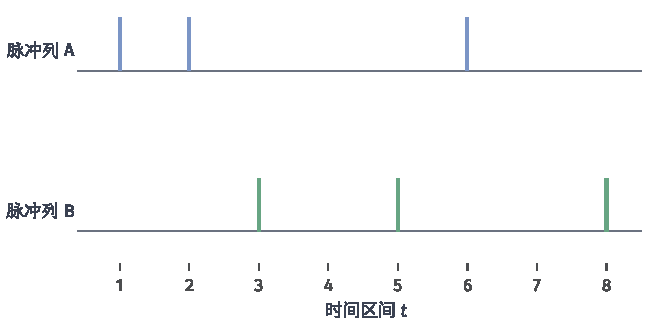
\includegraphics[width=\linewidth]{figures/03-models/02-neural-network-models/matplotlib/snn-codes/figure.pdf}
  \caption{两条构造的脉冲列在8个等宽时间区间内都发放3次，窗口频率相同，但首次发放位置和脉冲间隔不同。竖线表示事件，横轴为时间区间编号；频率读出只保留计数，时间读出还可使用排列。}
  \label{fig:snn-codes}
\end{figure}

输入编码与输出解码不必相同。网络可以接收时间戳事件，再用输出计数分类；也可以接收持续电流，通过输出单元的首次发放作决策。明确两端的约定，才能比较不同方案的精度和延迟。

\subsection{积分、泄漏与发放}
\label{sec:snn-neurons}

图~\ref{fig:snn-neuron-structure}将一个单元拆为突触响应、积分与泄漏、阈值检测和复位。输入事件只在到达时写入突触，突触响应与膜电位则保存连续值状态。输出脉冲反馈到复位路径，复位后的电位再经过一个时间步进入下一次积累；这条内部反馈解释了单个神经元也有记忆。
\begin{figure*}[htbp]
  \centering
  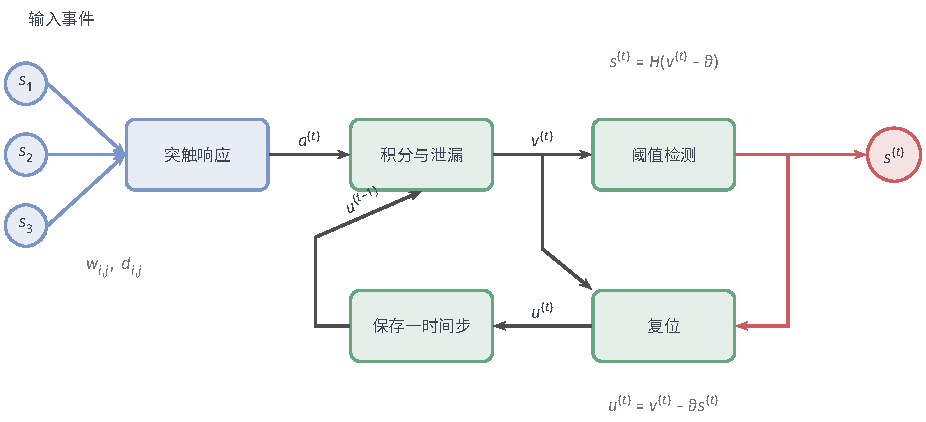
\includegraphics[width=\linewidth]{figures/03-models/02-neural-network-models/tikz/snn-neuron-structure/figure.pdf}
  \caption{离散脉冲神经元的计算结构。输入事件经带权突触形成输入增量$a^{(t)}$，红色模块完成积分、泄漏、阈值检测和复位，路径输出$s^{(t)}$。下方反馈保存复位后电位$u^{(t)}$，供下一步使用；$v^{(t)}$为复位前电位。图表示本章的更新次序，不表示细胞的解剖结构；突触自身也可保存状态，见式\eqref{eq:snn-synaptic-state}。}
  \label{fig:snn-neuron-structure}
\end{figure*}

一个输入脉冲常不足以触发输出。神经元需要累积输入，同时让旧输入的影响逐渐减弱。\term{膜电位}（membrane potential）是描述这种内部积累的状态变量；在简化人工模型中，它表示单元距离发放阈值还有多远，不要求逐项复现生物细胞的电化学过程。

\term{漏积分发放模型}（LIF）在两次发放之间用一阶动态描述积累与遗忘。设膜电位为$u_i(t)$，静息电位为$u_{\mathrm{rest}}$，输入电流为$I_i(t)$，膜时间常数为$\tau_m>0$，电阻为$R$，则
\begin{equation}
  \tau_m\frac{\mathrm d u_i(t)}{\mathrm d t}
  =-[u_i(t)-u_{\mathrm{rest}}]+RI_i(t)\text{。}
  \label{eq:snn-continuous-lif}
\end{equation}
无输入时，偏离静息电位的部分按$\exp(-\Delta t/\tau_m)$衰减。膜电位从下方达到阈值$\vartheta>u_{\mathrm{rest}}$时，模型产生一次脉冲并复位。\term{不应期}（refractory period）指发放后暂时不能再次发放的时间，可通过锁定状态或禁止发放来建模。微分方程、阈值检测、复位和不应期共同决定动态，不能只给方程就认为神经元已完整定义\scite{gerstner2014}

为便于训练，以下把静息电位移到0，并把电流及积分系数吸收到输入增量$a_i^{(t)}$中。采用先积分、再检测、再减去阈值的离散模型：
\begin{align}
  v_i^{(t)}&=\alpha u_i^{(t-1)}+a_i^{(t)},
  &\alpha&=\exp(-\Delta t/\tau_m),\label{eq:snn-discrete-integrate}\\
  s_i^{(t)}&=H(v_i^{(t)}-\vartheta),
  &H(z)&=\begin{cases}1,&z\geq0,\\0,&z<0,\end{cases}
  \label{eq:snn-discrete-fire}\\
  u_i^{(t)}&=v_i^{(t)}-\vartheta s_i^{(t)}\text{。}
  \label{eq:snn-soft-reset}
\end{align}
$v_i^{(t)}$为检测前电位，$u_i^{(t)}$为复位后电位，$\alpha\in(0,1)$控制相邻时间步之间的保留程度。此模型每步最多发放一次；若$v_i^{(t)}$远大于阈值，超出的电位会保留到后面，因此它不能精确表示任意高频的连续发放。时间步、输入尺度和发放上限必须配合选择。

式\eqref{eq:snn-soft-reset}称为减法复位，保留超过阈值的剩余电位。另一种\term{硬复位}（hard reset）直接将发放后的电位设为$u_{\mathrm{reset}}$，即$u_i^{(t)}=(1-s_i^{(t)})v_i^{(t)}+s_i^{(t)}u_{\mathrm{reset}}$。两种复位既改变前向轨迹，也改变反向传播。去掉泄漏、令$\alpha=1$，得到离散的\term{积分发放模型}（integrate-and-fire, IF）；增加适应变量或非线性电位项，可以描述更丰富的发放模式。模型越复杂，需要存储和更新的状态越多。

\begin{example}[相同输入在不同间隔下的结果]
  \label{ex:snn-integration}
  取$\alpha=0.8$、$\vartheta=1$、$u^{(0)}=0$，不设不应期。输入增量$(0.6,0.6,0,0.6)$依次给出检测前电位$(0.6,1.08,0.064,0.6512)$，输出为$(0,1,0,0)$，复位后电位为$(0.6,0.08,0.064,0.6512)$。第二步的两个近邻输入共同越过阈值，而第四步输入与前次积累相隔更远，不能触发发放。

  若将相同的三个$0.6$改放在第1、3、5步，中间输入为0，则检测前电位依次为$0.6,0.48,0.984,0.7872,1.22976$，只有第五步发放。总输入不变，输出时刻却改变了。这些数值展示泄漏与事件间隔的关系，不是生物测量或识别实验。
\end{example}

图~\ref{fig:snn-lif}把示例的第一组输入画成轨迹。发放由检测前电位决定，复位后的低电位则成为下一步的初始状态；把这两个时刻混在一起会误读阈值与输出的关系。
\begin{figure}[htbp]
  \centering
  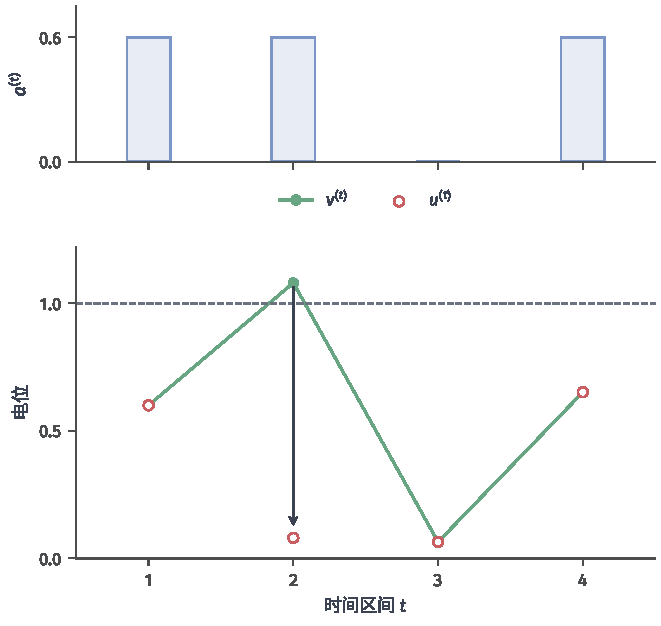
\includegraphics[width=\linewidth]{figures/03-models/02-neural-network-models/matplotlib/snn-lif/figure.pdf}
  \caption{示例~\ref{ex:snn-integration}的离散LIF计算。蓝色竖线表示输入增量，红色实线连接检测前电位$v^{(t)}$，黄色空心圆为复位后电位$u^{(t)}$，虚线为阈值；第二步检测后发放并减去1。连线帮助比较离散状态，不表示步间的连续电位轨迹。}
  \label{fig:snn-lif}
\end{figure}

LIF保留了积累与遗忘，但固定阈值不表达“刚刚频繁发放后变得较难继续发放”。可以增加适应迹$r_i^{(t)}$，例如
\begin{equation}
  r_i^{(t)}=\rho r_i^{(t-1)}+s_i^{(t-1)},\qquad
  \vartheta_i^{(t)}=\vartheta_0+\kappa r_i^{(t)},
  \quad 0\leq\rho<1,\quad\kappa\geq0\text{。}
  \label{eq:snn-adaptive-threshold}
\end{equation}
过去发放暂时抬高阈值，适应迹随后衰减；替换式\eqref{eq:snn-discrete-fire}中的阈值即可形成一种适应LIF模型。额外状态延长动态时间尺度，也增加反向路径和存储。更复杂的神经元可以使用适应电流、非线性膜电位或离子通道状态。例如，\term{自适应指数积分发放}（adaptive exponential integrate-and-fire, AdEx）模型结合膜电位的指数非线性与适应电流。表~\ref{tab:snn-neuron-models}比较这些模型保留的动态细节。
\begin{table*}[htbp]
  \centering\small
  \begin{tabularx}{\linewidth}{@{}
    >{\raggedright\arraybackslash}p{34mm}
    >{\raggedright\arraybackslash}p{49mm}
    >{\raggedright\arraybackslash}X@{}}
    \toprule
    神经元模型 & 主要状态与发放机制 & 适用关注点 \\
    \midrule
    积分发放（IF） & 膜电位积分，阈值与复位 & 简化计数对应，未包含泄漏 \\
    漏积分发放（LIF） & 膜电位积累与泄漏，阈值与复位 & 有限时间记忆与较低单元复杂度 \\
    适应LIF & 膜电位及适应迹，动态阈值或电流 & 发放历史改变后续响应 \\
    自适应指数积分发放（AdEx） & 膜电位非线性及适应电流 & 以较少状态描述丰富发放模式 \\
    Izhikevich模型 & 膜电位与恢复变量，阈值复位 & 以简化二维动态模拟多种放电行为 \\
    单室Hodgkin--Huxley & 膜电位与离子通道门控变量 & 解释动作电位产生的电流机制 \\
    \bottomrule
  \end{tabularx}
  \caption{神经元模型按保留的动态细节比较。IF与LIF还需规定复位、不应期及时间离散化；表中不计另行添加的突触和延迟状态。复杂度更高的模型能表达更多细节，不自动产生更好的任务预测。}
  \label{tab:snn-neuron-models}
\end{table*}
\FloatBarrier

模型选择需要与问题一致。若只需积累事件形成分类分数，单室离子通道方程可能增加不必要的模拟成本；若研究动作电位波形或不同电流的作用，只报告LIF脉冲次数又不足以回答问题。模型参数的物理单位、输入尺度与数值步长应配套，不能在不同神经元中直接沿用同一组数值\scite{gerstner2014}

\subsection{网络连接与状态传播}
\label{sec:snn-connections}

图~\ref{fig:snn-connections}比较相同单元的两种组织。前馈边将事件送到下一层，每个单元的膜电位仍跨时间保留；循环边再把网络过去的发放送回当前计算。循环与非循环说明的是单元之间的拓扑，不取消单元内部的状态递推。
\begin{figure*}[htbp]
  \centering
  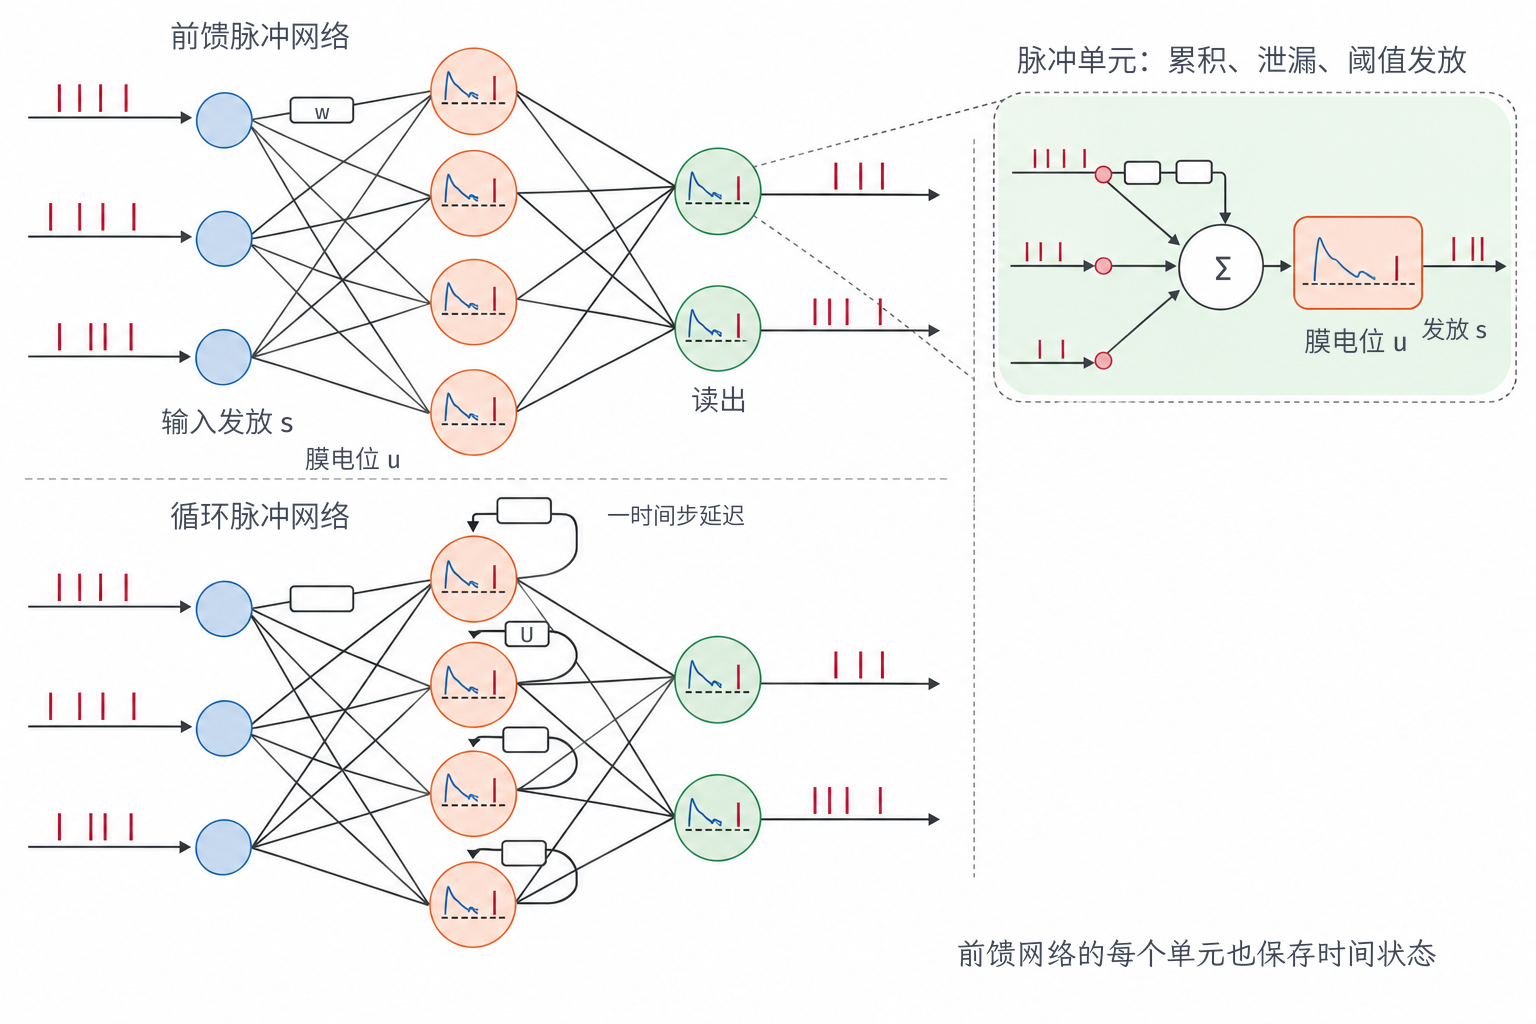
\includegraphics[width=\linewidth]{figures/03-models/02-neural-network-models/generated/snn-connections/figure.png}
  \caption{脉冲前馈网络与循环网络的构造性比较。单元内的膜电位轨迹表示内部状态，箭头传递离散发放，右侧给出输出读出。上半部只保留层间前馈连接；下半部增加使用上一时间步脉冲的循环边$\bm U$。边还可带权重与传播延迟，图中只标出一条代表连接。神经元数和连边用于说明结构，不对应训练模型。}
  \label{fig:snn-connections}
\end{figure*}

神经元之间的连接将发放事件变为后续单元的输入。\term{突触}（synapse）在这里指带权连接及其对接收状态的作用。最简单的离散突触把一个到达脉冲转为电位增量$w_{i,j}$：正权重促使接收单元接近阈值，负权重使其远离阈值。生物兴奋性、抑制性细胞对连接符号有更强约束；允许同一人工单元任意使用正负输出权重，是建模选择。

输入的作用还可以延续多个时间步。设一层有$m$个神经元，上层有$d$个，突触状态为$\bm q^{(t)}\in\mathbb R^m$，前馈权重为$\bm W\in\mathbb R^{m\times d}$，循环权重为$\bm U\in\mathbb R^{m\times m}$，偏置为$\bm b\in\mathbb R^m$，可写为
\begin{equation}
  \bm q^{(t)}=\beta\bm q^{(t-1)}
    +\bm W\bm s_{\mathrm{in}}^{(t)}
    +\bm U\bm s^{(t-1)}+\bm b,\qquad
  \bm a^{(t)}=\bm q^{(t)}\text{，}
  \label{eq:snn-synaptic-state}
\end{equation}
其中$\beta\in[0,1)$控制突触响应的衰减。脉冲是瞬时输入，$\bm q^{(t)}$与$\bm u^{(t)}$却可以继续保存历史。使用上一时间步的循环脉冲避免同一步的代数环；前馈层则可按层顺序读取本步输入。

更一般地，令$d_{i,j}\in\{0,1,2,\ldots\}$表示边$j\to i$的总传播延迟，以离散时间步计，实际延迟为$d_{i,j}\Delta t$。权重为$w_{i,j}$的边贡献$w_{i,j}s_j^{(t-d_{i,j})}$；式\eqref{eq:snn-synaptic-state}中的前馈边对应$d_{i,j}=0$，循环边对应$d_{i,j}=1$。为保持显式更新，每个反馈回路的总延迟必须至少为一步；零延迟边组成的子图必须无环，才能按拓扑顺序读取本步已经算出的脉冲。若允许零延迟自反馈，例如$s=H(2s-1)$，则$s=0$与$s=1$都满足方程，已知历史就不能唯一决定本步输出。实现还需维护尚未到达的事件，并为序列起点以前的脉冲指定初始历史。

即使没有循环边，脉冲神经元本身也有跨时间状态，所以脉冲前馈网络不是无记忆的逐帧映射。加入循环边后，状态既保存本单元的积累，又接收其他单元的历史发放。初始状态、序列边界、延迟和同时到达事件的处理次序都属于模型定义；独立样本常重置状态，持续流则通常保留状态。

\section{参数学习}
\label{sec:snn-learning}

给定发放机制后，还需要决定怎样调整连接，使输出与任务相符。三条路线使用的信息不同：局部规则根据相邻活动更新突触；端到端训练根据任务损失调整参数；转换方法先学习连续值网络，再把它的激活解释为脉冲统计量。它们可以组合，但优化的对象和误差来源不能混同。

下面的基本例子把泄漏、阈值和时间常数视为已给定参数，主要学习连接权重与读出。也可以学习这些动态参数，例如用Sigmoid参数化泄漏因子、用正值变换参数化阈值，以维持模型约束；此时梯度还要沿相应动态路径传播。整数传播延迟不能直接按普通实数参数求导，需另行设计搜索或可微近似。

\subsection{局部可塑性规则}
\label{sec:snn-plasticity}

如果只允许一个突触读取连接两端的活动，更新就无法直接使用全网反向传播的误差信号。\term{赫布学习}（Hebbian learning）根据输入端与输出端的共同活动调整连接，表达“共同活跃时加强联系”的局部相关性思想。一个简化规则为$\Delta w_{i,j}=\eta x_jy_i$，其中$x_j,y_i$是同一观察窗口的活动量，$\eta>0$为更新系数。持续相关活动可能令权重不断增大，因此通常还需衰减、归一化、竞争或上下界。

共同活动的窗口并没有区分先后。\term{脉冲时序依赖可塑性}（spike-timing-dependent plasticity, STDP）进一步依据突触前后发放的时间差更新权重。令$\Delta t=t_{\mathrm{post}}-t_{\mathrm{pre}}$，一种典型的成对教学规则为
\begin{equation}
  \Delta w_{i,j}=\begin{cases}
    A_+\exp(-\Delta t/\tau_+),&\Delta t>0,\\
    -A_-\exp(\Delta t/\tau_-),&\Delta t<0,
  \end{cases}
  \label{eq:snn-stdp}
\end{equation}
其中$A_+,A_->0$为幅度，$\tau_+,\tau_->0$为时间尺度，同时发放时另定规则。该形式把“输入先到、输出随后发生”与相反次序区分开。实验中的变化还取决于细胞类型、突触强度和发放组合，不能把这条成对指数曲线当成全部生物可塑性的统一规律\scite{bi1998}

局部计算不必保存所有事件对。可以用指数衰减的活动迹记录近期发放，突触后发放时读取突触前迹来加强权重，突触前发放时读取突触后迹来减弱权重。采用所有配对还是最近邻配对、权重是否有界，会产生不同学习动态。

局部相关性与分类正确率仍有距离：频繁共同出现的输入未必是区分标签所需的特征。为把局部活动与任务结果连接，可加入第三个调制信号，令$\Delta w_{i,j}=\eta m^{(t)}e_{i,j}^{(t)}$。其中$e_{i,j}^{(t)}$是记录近期局部活动及可更新程度的\term{资格迹}（eligibility trace），$m^{(t)}$传递奖励、误差或其他全局调制。第三因素能改变更新方向和时机，但它是否等价于目标函数梯度，还要检查调制信号和资格迹的具体构造\scite{gerstner2018plasticity}

\subsection{替代梯度与时间反向传播}
\label{sec:snn-surrogate}

监督任务需要将输出误差分配到多层连接。设每个样本含$K$步输入脉冲，标签为$y$，输出读出为$\bm z=K^{-1}\sum_t\bm s_{\mathrm{out}}^{(t)}$，可以用$\ell(\bm z,y)$训练分类器。其他读出可使用膜电位、过滤后的输出或发放时间；读出改变时，损失及其求导也应同步改变。

困难在式\eqref{eq:snn-discrete-fire}的阶跃函数。$H$在阈值之外的普通导数为0，阈值处不连续。直接将其导数带入链式法则，几乎处处得不到能调整发放的信号；小幅改变权重还可能在越过阈值时突然改变整条轨迹。\term{替代梯度}（surrogate gradient）在前向计算中保留离散发放，在反向计算中用一个有限、非零的函数代替阶跃导数。例如，令$z=v-\vartheta$，使用
\begin{equation}
  \frac{\partial s}{\partial v}\ \rightsquigarrow\
  \psi(z)=\frac{c}{(1+\kappa|z|)^2},\qquad c,\kappa>0\text{。}
  \label{eq:snn-surrogate-derivative}
\end{equation}
符号$\rightsquigarrow$表示指定替代规则，不表示真实导数相等。靠近阈值的单元收到较强训练信号，远离阈值的单元收到较弱信号。$c$改变梯度幅度，$\kappa$改变有效宽度；两者与阈值及电位尺度有关\scite{neftci2019surrogate}

替代规则也进入复位的导数。对本章的减法复位，若不停止复位路径的求导，有
\begin{equation}
  \frac{\partial u_i^{(t)}}{\partial v_i^{(t)}}
  \ \rightsquigarrow\ 1-\vartheta\psi(v_i^{(t)}-\vartheta)\text{。}
  \label{eq:snn-reset-gradient}
\end{equation}
若实现中把复位脉冲视为常数，这个导数改为1。它们前向相同，反向却不同；硬复位的表达式也要单独求导。说明训练方法时，应明确复位是否参与反向计算，不能只写“使用替代梯度”。

图~\ref{fig:snn-surrogate-forward-backward}将真实前向发放与指定的反向规则放在同一计算链上。两种复位导数约定共享前向状态更新，区别只进入回传。

\begin{figure*}[htbp]
  \centering
  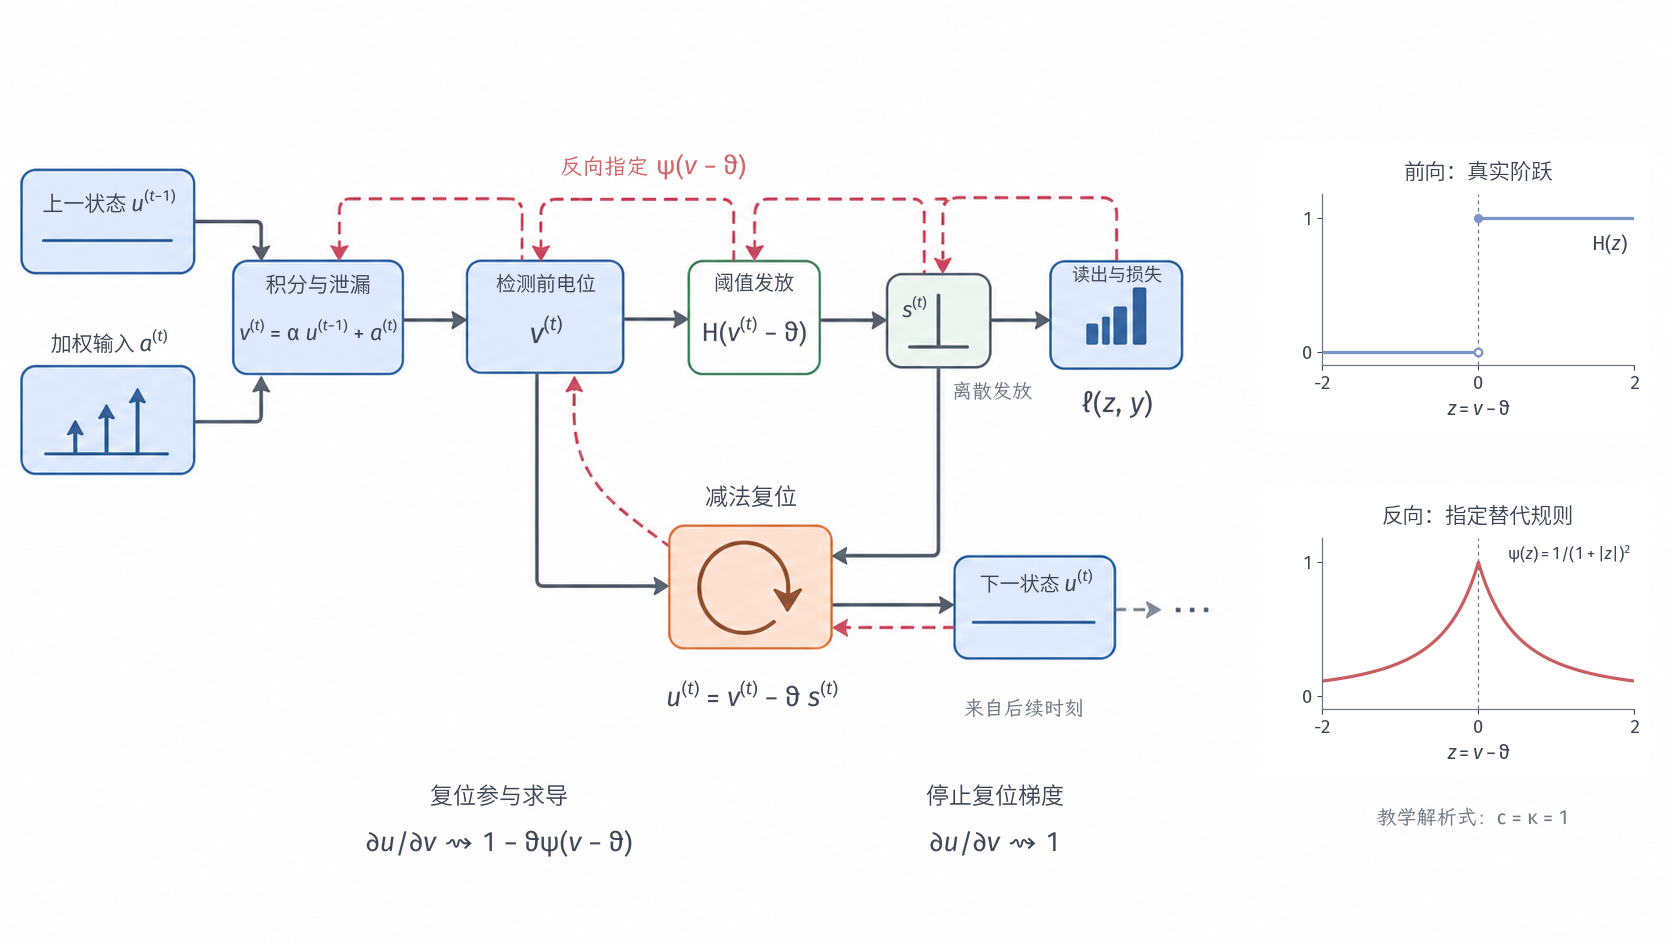
\includegraphics[width=\linewidth]{figures/03-models/02-neural-network-models/generated/snn-surrogate-forward-backward/figure.png}
  \caption{LIF前向计算与替代梯度。前向使用真实阶跃发放和减法复位；反向在发放处指定替代规则$\psi$。右侧解析曲线取$c=\kappa=1$，阶跃在零处取一；下方两式分别表示复位参与求导与停止复位梯度，两种约定不改变前向发放。}
  \label{fig:snn-surrogate-forward-backward}
\end{figure*}

将$\bm q^{(t)}$、$\bm u^{(t)}$和所需延迟状态合并为$\bm h^{(t)}$，网络可写为$\bm h^{(t)}=F_{\bm\theta}(\bm h^{(t-1)},\bm x_t)$。第\ref{chap:recurrent-networks}章的时间展开和共享参数梯度累积因此仍然适用。区别在于发放及相关路径的局部导数由替代规则指定。梯度需要跨层和跨时间传播，较长窗口增加激活存储，截断展开则遗漏被切断的历史影响。替代梯度通常既不是原离散网络损失的精确梯度，也不保证是某个统一平滑目标的梯度；它是一种有用但需要验证的学习近似。

\begin{algorithm}[脉冲网络的监督训练]
  \label{alg:snn-supervised}
  \begin{algorithmic}[1]
    \Require 输入序列与标签、时间步数$K$、神经元参数、替代规则$\psi$
    \Ensure 学得的权重与读出参数
    \For{每个训练小批量}
      \State 按样本边界设置膜电位、突触状态和延迟队列
      \For{$t=1,\ldots,K$}
        \State 计算突触输入，按式\eqref{eq:snn-discrete-integrate}--\eqref{eq:snn-soft-reset}更新各层
        \State 保存反向计算所需状态并积累输出读出
      \EndFor
      \State 由读出与标签计算损失
      \State 沿展开图反向计算，以$\psi$代替发放导数并采用约定的复位导数
      \State 累积共享参数梯度，必要时裁剪，再更新参数
    \EndFor
  \end{algorithmic}
\end{algorithm}

\subsection{人工网络到脉冲网络的转换}
\label{sec:snn-conversion}

频率编码提供了另一条学习路径：先训练具有非负激活的连续值网络，再用发放率近似这些激活。\term{人工网络到脉冲网络转换}（ANN-to-SNN conversion）就是建立连续激活与脉冲统计量的对应，以复用已经学得的权重。理解这一对应，可以从不泄漏的积分发放模型开始。

设$\alpha=1$、$u^{(0)}=0$，采用减法复位，每步输入增量为$a^{(t)}$，将$K$次状态更新求和得
\begin{equation}
  \vartheta\sum_{t=1}^{K}s^{(t)}
  =\sum_{t=1}^{K}a^{(t)}-u^{(K)}\text{。}
  \label{eq:snn-conversion-balance}
\end{equation}
若输入非负且每步不超过$\vartheta$，则$0\leq u^{(K)}<\vartheta$，于是
\begin{equation}
  0\leq\frac1K\sum_{t=1}^{K}a^{(t)}
       -\frac{\vartheta}{K}\sum_{t=1}^{K}s^{(t)}
  <\frac{\vartheta}{K}\text{。}
  \label{eq:snn-conversion-error}
\end{equation}
这说明阈值乘以平均发放量可以近似平均输入，剩余电位造成有限窗口误差。比如恒定输入0.3、阈值1、窗口4步，只发放1次，对应平均值0.25，尚有0.2电位未释放。窗口10步恰好发放3次，对应0.3。这里是输入已校准的单神经元结论，不能直接作为多层网络的统一误差界。

实际转换需处理负激活、偏置、归一化和不同层的尺度。对线性层$\bm W\bm x+\bm b$，若训练后的BatchNorm使用固定均值$\mu$和方差$\sigma^2$，它的仿射变换可以折叠到权重与偏置。对输出通道$i$，有$\bm W'_{i,:}=\gamma_i\bm W_{i,:}/\sqrt{\sigma_i^2+\epsilon}$，$b'_i=\gamma_i(b_i-\mu_i)/\sqrt{\sigma_i^2+\epsilon}+\zeta_i$。这里$\gamma_i,\zeta_i$为归一化的缩放和偏移，折叠使用推理统计量。阈值或层权重再依据代表性校准数据调节，使常见激活既不会长期静默，也不会超出单步发放上限\scite{rueckauer2017conversion}

加入泄漏后，式\eqref{eq:snn-conversion-balance}会多出遗忘项；采用硬复位还会丢弃超阈值的剩余电位。多层的有限窗口误差、上游发放延迟和统计尺度偏差都可能累积。转换适合能够由非负发放统计量近似的计算；若目标依赖精确相对时序，仅保留连续激活的频率对应通常不够。端到端脉冲训练则可以直接针对目标窗口和读出来调整动态。

\section{理论分析}
\label{sec:snn-analysis}

\subsection{时序表达与动态稳定性}
\label{sec:snn-temporal-stability}

脉冲网络能否区分输入，需要同时考察编码、状态和读出。若编码只给出窗口计数，原始时间顺序已经丢失，后续网络无法从计数恢复它。若编码保留时刻，有限时间常数又可能让相隔很远的事件互不影响。即使内部状态不同，最终只做总计数的读出也可能把两条轨迹合并。表达能力属于整个输入到输出的映射，不能只数神经元或脉冲模式。

在不跨越阈值、发放模式固定的区间，LIF状态差异会按泄漏因子衰减：相同后续输入下，单元满足$\delta u^{(t)}=\alpha\delta u^{(t-1)}$。但阈值附近的小扰动可能使某一步多发放一次，继而改变复位、突触输入和后续事件。因而$\alpha<1$只说明无发放切换时的泄漏稳定性，不足以保证整个循环脉冲网络全局收缩。

分析一段固定发放模式内的连续状态递推，可以像第\ref{chap:recurrent-networks}章一样检查局部Jacobian矩阵连乘。遇到阈值切换时，还需处理不连续映射、事件时刻的变化和复位。训练用的替代Jacobian矩阵则描述指定的反向规则，不能直接用它证明真实离散动态的稳定性。较强泄漏有利于忘记过时状态，也缩短可利用的历史；循环反馈、延迟和适应状态可以改变这种取舍。

\subsection{精度、延迟与事件数量}
\label{sec:snn-cost}

时间离散化和编码共同决定可表示的精度。若用$K$步中的脉冲比例表示$[0,1]$内数值，读出的间隔为$1/K$；随机编码还叠加抽样方差。首次发放编码可以只用一个事件表示多个时间位置，但接收端必须等待该事件，并能区分这些位置。减少事件数与缩短决策时间是两个不同目标。

设一次推理中神经元$j$发放$N_j$次，连接到$d_j$个接收突触，若每次发放都访问这些连接，则触发的突触累加数为
\begin{equation}
  C_{\mathrm{syn}}=\sum_jN_jd_j\text{。}
  \label{eq:snn-event-cost}
\end{equation}
这个量比“发放次数”更接近通信和突触处理成本。一个发放稀少却有大量扇出的单元，仍可能触发很多操作。按时间步模拟$m$个状态单元还需$O(Km)$次状态更新，若实现为稠密矩阵计算，未发放的连接也未必被跳过。事件驱动实现可以在到达事件时更新部分状态，但仍需处理泄漏、内部发放和延迟队列。

因此，SNN的能耗不能由二值输出或事件数单独推出。评估应同时给出任务质量、观察窗口、决策延迟、突触访问量、状态存储及实际设备上的能耗。与连续值网络比较时，还要统一输入预处理和决策条件。稀疏事件提供节省操作的机会，最终收益取决于数据活动、网络连接和硬件是否能利用这种稀疏性。

\section{常见应用}
\label{sec:snn-applications}

\subsection{事件流识别}
\label{sec:snn-event-recognition}

变化驱动的视觉传感器为脉冲网络提供了直接的事件输入。\term{事件相机}（event camera）在像素亮度变化达到阈值时输出位置、时刻和变化方向，而非在固定间隔输出整帧图像。一个样本可表示为事件序列$\{(x_k,y_k,t_k,p_k)\}_{k=1}^{n_e}$，其中$(x_k,y_k)$为像素坐标，$t_k$为时间戳，$p_k\in\{-1,1\}$为亮度变化极性。事件说明变化，并不直接给出完整的绝对亮度图像\scite{lichtsteiner2008sensor}

以动作片段分类为例，可以按像素和极性分输入通道，将时间戳划入宽度$\Delta t$的区间，得到输入脉冲张量。如果同一像素在一个区间多次触发，可采用事件计数，或缩短区间以保留二值表示；合并事件会改变信息。空间卷积连接提取局部变化模式，膜电位与突触状态累积时间关系，再用类别输出单元的计数或连续读出产生分数。

若类别$c$的计数为$N_c$，可以取$z_c=N_c/K$并用Softmax交叉熵训练，预测为$\argmax_c z_c$；所有计数为0时要规定平局处理或继续观察。损失可以只在片段结束计算，也可以在多个截断窗口计算以训练较早输出。后者需要固定评价时刻，避免把使用更多未来事件的模型与早期决策模型直接比较。

数据划分应以独立动作片段、主体或采集场景为单位，不能把同一连续记录切出的相邻窗口随机分到训练和测试中。事件噪声、场景变化与传感器阈值都会改变输入分布，识别结果须在规定的时间预算下评估。

\subsection{连续感知与动态响应}
\label{sec:snn-continuous-response}

持续感知没有天然的片段终点。网络接收不断到来的变化，保留状态，并在预定时刻或满足决策条件时产生输出。比如一个教学性的运动方向检测器可以用两组位置通道接收事件，利用不同突触延迟使某一方向的事件在下游同时到达；相反方向则不形成同样的时间重合。LIF的积累与阈值把这种重合转为发放，方向读出据此给出分数。

连续输出也可以从过滤后的状态得到。设$m$维输出脉冲为$\bm s^{(t)}$，令$\bm r^{(t)}=\rho\bm r^{(t-1)}+(1-\rho)\bm s^{(t)}$，$\rho\in[0,1)$，再用$\hat{\bm y}^{(t)}=\bm C\bm r^{(t)}+\bm d$预测连续量。$\rho$越大，输出越平滑，也越迟缓；用膜电位读出则会保留阈值以下的状态。输出形式应服从任务对响应速度、抖动和置信度的要求。

持续状态还会带来边界问题。静默期间应让历史影响按模型衰减；传感器重启、场景切换或长时间中断后，可以按明确规则重置状态。训练时若每个短窗口都重置，使用时却无限保留状态，网络面对的状态分布可能不同。保留跨窗口状态时，也要说明哪些梯度被截断，不能把跨窗口记忆误认为已经完成跨窗口信用分配。

\section{本章小结}
\label{sec:snn-summary}

SNN以离散发放通信、以连续状态保存历史，编码、突触、泄漏、阈值与读出共同形成预测。局部规则、替代梯度和网络转换分别利用相邻活动、近似任务梯度与发放统计对应。较长窗口能改善部分编码精度，也增加延迟与操作；实际收益仍须连同输入编码、突触访问、状态更新和设备测量判断。
